\documentclass[12pt]{article}
\usepackage{fancyhdr}
\usepackage{lastpage}
\usepackage{geometry}
\usepackage{amsmath}
\usepackage{setspace}
\usepackage{graphicx}
\usepackage{caption}
\geometry{a4paper,scale=0.8}
\pagestyle{plain}
\renewcommand{\headrulewidth}{0.4pt}
\renewcommand{\footrulewidth}{0.4pt}
\setlength{\baselineskip}{23pt}


\begin{document}
	\thispagestyle{plain}
	\noindent \Large \textbf{The Fama-French Three-Factor Model, Revisited}\\ \\
	\noindent Jin, Kim, Quek, Wang and Woon (2019)\\
	\noindent \normalsize \textit{Singapore Management University, Singapore}\\ \\
	\noindent May 2019, working paper, final version pending
	
		\section{Abstract} % Numbered section
	
		This paper outlines the results of a validity test we have conducted on the Fama and French (1993) three-factor model on eligible stocks listed in NYSE, NASDAQ and AMEX for the period between July 2011 to December 2018 (the sample period). After conducting our analysis and running several statistical tests, we have arrived at the conclusion that Fama and French (1993) three-factor model continues to display extremely significant explanatory power over U.S. stock returns (proxied by the returns on our constructed quintile-based portfolios) during the sample period. We also found the three-factor model to be superior to the one-factor CAPM in terms of explanatory power over U.S. stock returns during the sample period. However, we found that the Small Minus Big (SMB) and the High Minus Low (HML) factors can be slightly lacking in terms of statistical significance when it comes to a few of our constructed quintile-based portfolios, although the overall adjusted R-squared values of the regression studies on those quintile-based portfolios remain significant. Further, in contrast to the findings published by Fama and French (1993), we found that Big companies displayed higher mean returns than Small companies over the sample period (negative mean SMB), with said mean excess return being statistically significant at the 5\% level. Companies with Low book-to-market equity were also observed to have displayed higher mean returns than those with High book-to-market equity (negative mean HML) though this was found to be statistically insignificant at the 5\% level. A deeper dive into the divergence of our observed mean SMB and HML readings from those observed by Fama and French (1993) revealed a noteworthy shift away from thematic "long SMB" and "long HML" plays over the recent decade.
	
	\section{Introduction \& Literature Review} % Numbered section
	
	The emergence of Modern Portfolio Theory introduced by Markowitz (1952) has set the foundation for portfolio management research, and has spurred an outpouring of research of a similar focus. The Capital Asset Pricing Model (CAPM) developed by harpe (1964), Lintner (1965) and Black (1972) is a result of such an outpouring. The CAPM attempts to explain stock returns using excess market returns as an all-encompassing risk factor, an idea which was quickly popularised, but has since been met with much scrutiny and many empirical contradictions. Amongst the critics of the CAPM are Fama and French (1993), who have built a case arguing that market excess returns alone do not fully explain cross-sectional variations in equity returns and that the addition of two empirically-backed factors are better explaining said variations. The model is also known as the Fama and French (1993) three-factor model:
	
	$$
	R(t) - R_f(t) = a+ b(R_{mkt} - R_f) + s(SMB) + h(HML) +\epsilon_i
	$$
	
	\noindent The three-factor model introduced by Fama and French (1993) has come a long way in shaping views about drivers of stock returns in academia and in practice. On top of the market $\beta$ factor proposed and popularised by Sharpe (1964), Lintner (1965) and Black (1972) in their Capital Asset Pricing Model (CAPM), Fama and French (1993) proposed two additional and empirically-backed factors for the explanation of stock returns: Size (ME) and Book-to-Market Equity (BE/ME). \\
	
	\noindent The three-factor model was proposed in response to several discovered empirical contradictions to the CAPM highlighted in Fama and French (1992a). For one, Banz (1981) found that Size (proxied by Market Equity, or ME) adds explanatory power to cross-sectional average returns provided by market $\beta$s. Also, Bhandari (1988) found a positive relationship between firm leverage and average stock returns. To add, Rosenberg, Reid and Lanstein (1985) and Stattman (1980) discovered a positive relationship between Book-to-Market Equity and average U.S. stock returns. Further, Basu (1983) found that earning-price ratios (E/P) help in the explanation of cross-sectional U.S. stock returns when used in conjunction with size and market $\beta$ factors. These findings contradict the viewpoint that market $\beta$s alone are sufficient in describing cross-sectional expected stock returns. \\
	
	\noindent Amongst the potential and empirically-backed factors for stock returns mentioned earlier, Fama and French (1992a) found that Size (ME) and Book-to-Market (BE/ME), when used together, appear to absorb the roles played by leverage and E/P as explanatory factors for stock returns. it was also discovered that Size and Book-to-Market are able to well-explain cross-sectional average returns for stocks listed on the NYSE, Amex and NASDAQ for the period between 1963 to 1990. This discovery laid the groundwork for the three-factor model proposed by Fama and French (1993).\\
	
	\noindent In their study, Fama and French (1993) divided eligible common stocks traded on the NYSE, Amex or NASDAQ into six portfolios based on their Size and Book-to-Market Equity. Size was proxied by Market Equity (ME), and stocks were determined to be Big (B) or Small (S) based on whether they were above or below the median NYSE ME. Stocks were also determined to have Low (L), Medium (M) or High (H) Book-to-Market Equity based on whether they belonged to the bottom 30\%, middle 40\% or top 30\% of NYSE BE/ME. The resulting six portfolios formed were: S/L, S/M, S/H, B/L, B/M and B/H. Monthly Size (SMB) and Book-to-Market Equity (HML) factor readings were then constructed from the returns of these six portfolios. The Market factor was proxied by $R_M - R_F$, where $R_M$ is the result of the value-weighted return of eligible common stocks and $R_F$ is the one-month U.S. Treasury bill rate. Data relating to the study were obtained from the CRSP and COMPUSTAT.\\
	
	\noindent Fama and French (1993) then proceeded to use the same eligible stocks (used in the SMB and HML factor constructions) to construct 25 portfolios based on their Size and Book-to-Market Equity quintiles. The monthly excess returns of these 25 portfolios were then used as the dependent variables for regressions against the Market, Size and Book-to-Equity factors (the independent variables). It was found that, when used together, the three stock market factors were able to explain most of the variation in the returns of the 25 portfolios.\\
	
	\noindent It was also found that the SMB slope coefficients decreased monotonically as portfolio Size increased, whilst the HML slope coefficients increased monotonically as portfolio Book-to-Market Equity increased. Further, the regression intercepts were found to be mostly statistically indifferent from zero. On the other hand, when the Market factor was the only independent variable in the regressions, lower $R^2$ values were obtained and the Size effect seen in the intercepts discovered by Banz (1981) appeared. Overall, the results of the study offered compelling evidence in support of Size and Book-to-Market Equity as additional explanatory factors for stock returns.\\
	
	\noindent With all that said, the three-factor model is not without its criticisms. For instance, Daniel and Titman (1997) argued that it is the firm characteristics (e.g. region, industry, related lines of business etc), not the covariance structure of returns that actually explain the cross-sectional variation in stock returns. Daniel and Titman (1997) discovered that, once firm
	characteristics were controlled for, expected returns did not seem to be positively related to Market, SMB and HML loadings. The study was conducted for returns over 20.5 years between July 1973 to December 1993. Davis, Fama and French (2000), however, rebutted with their own findings with a higher-powered test, owing to a longer test period of 68 years between July 1929 and June 1997.\\
	
	\noindent Further, a plethora of subsequent studies successfully replicating the insights obtained from Fama and French (1993) for different regions and for different time periods have lent further credence to the notion that the Size and Book-to-Market Equity factors are indeed viable additions to the Market factor as explainers of stock returns.\\
	
	\noindent In recent times, there have been motivations to add more risk factors onto the original Fama and French (1993) three-factor model. Fama and French (2015) extended their original three-factor model by suggesting two additional factors: profitability (Robust Minus Weak, RMW), and investment, (Conservative Minus Aggressive, CMA). There have also been several calls elsewhere to add other risk factors such as momentum and low-volatility as part of the original three-factor model. \\
	
	\noindent Regardless, we are inspired to validate the original Fama and French (1993) three-factor model, albeit in a more modern time, between July 2011 to December 2018. As such, our research null hypothesis is as follows:\\
	
	``\textit{The three stock-market factors suggested by Eugene F. Fama and Kenneth R. French in their 1993 paper titled “Common Risk Factors in the Returns on Stocks and Bonds” do not significantly explain the returns of stocks listed on the NYSE, NASDAQ and AMEX for the period between July 2011 and December 2018.}" \\

	\noindent which if disproved, further validates the findings of Fama and French (1993), even in today's age.
	
\newpage
		
\section{Data, Research Design \& Methodology}
\noindent \textbf{Research Sample}\\
\noindent Our data sample includes data on all eligible stocks listed on the NYSE, NASDAQ and AMEX for the period between July 2011 to December 2018 (the sample period). Monthly data was used to calculate factor realisations and portfolio returns. In our deeper dive into the Small Minus Big (SMB) and the High Minus Low (HML) factors, we broadened our sample period to be between Jan 1929 and December 2018 (the extended sample period) and utilised pre-computed Fama-French factors and portfolio returns provided by Wharton Research Data Services (WRDS).\\

\noindent \textbf{Data Source: Wharton Research Data Services (WRDS)}\\
Wharton Research Data Services (WRDS) provided us with the following necessary databases Fama and French (1993) utilised in their original study: Center for Research in Security Prices (CRSP), Compustat - Capital IQ, the CRSP/Compustat Merged Database (CCM) and Fama-French Portfolios and Factors. \\

\noindent \textbf{Center for Research in Security Prices (CRSP)}\\
\noindent The Center for Research in Security Prices (CRSP) provided us with relevant data on the monthly closing price, returns and outstanding number of eligible stocks. We used PERMCOs and PERMNOs as unique entity and issue identifiers when navigating the CRSP database.\\

\noindent \textbf{Compustat - Capital IQ}\\
\noindent Compustat provided us with relevant data on total stockholders' equity, deferred taxes, investment tax credit and the book value of preferred stock. We used GVKEY as unique entity-level identifiers when navigating the Compustat database.\\

\noindent \textbf{CRSP/Compustat Merged Database (CCM)}\\
\noindent A common misconception is that the CCM database has seamlessly merged CRSP stock market data with Compustat accounting data. We found that this is not the case. The CCM database merely allows for Compustat-included data items to be searched for and linked with CRSP's PERMNO and PERMCO at the issue and entity level respectively, though it was found that GVKEYs and PERMCOs are not exclusive to each other. This means that a GVKEY may correspond to many PERMCOs and vice versa. \\

\noindent Thus, obtaining a complete data link between CRSP and Compustat data required an additional step of creating a new, truly unique entity-level identifier. A new identifier called "GVKEY PERMCO" was created for purposes of traversing between datasets.
For example, if Apple Inc’s GVKEY is 1690 and its PERMCO is 7, its GV KEY PERMCO is 16907, which is a unique identifier. Eventually, the CCM was used only for purposes of matching GVKEYs to PERMCOs, then raw data was obtained from standalone datasets.\\

\noindent \textbf{Factor Construction}\\
$$
R_{i_t}-R_{f_t}=\alpha_{it}+b_{it}(R_{M_t}-R_{f_t})+s_{i_t}(SMB)+h_{i_t}(HML)+\epsilon_{i_t}
$$

\newpage

\noindent \textbf{Rm-Rf}\\
The excess portfolio return in month t, $(R_{M_t}-R_{f_t})$, is the excess market portfolio return in month t. The market return for month t, $R_m$, was simply proxied by the average of return all eligible stocks, weighted by market capitalisation. Additionally, 1-month T-bill rates were used as a proxy for the risk free rate.\\

\noindent \textbf{BE and ME}\\
Using data obtained from both CRSP and COMPUSTAT (which was further validated by Bloomberg data) we computed the following items:

\begin{itemize}	
\item{Market Common Equity (ME) = Market Capitalisation of the Firm at December of time t-1.}
\item{Book Equity = Book Value of Common Equity + Book Value of Preferred Stocks}
\item{Book Values of Common Equity  = (Total Stockholders’ Equity + Deferred Taxes + Investment Tax Credit – Book Value of Preferred Stock) of the Firm at time t-1.}
\item{Book Value of Preferred Stocks = Redemption, Liquidation or Carrying Value of Preferred Stock, in that order, when available.}
\end{itemize}

 \noindent From these, the book-to-market (BE/ME) ratio of each stock for each year was computed. For each year, all eligible stocks (traded on the NYSE, NASDAQ or Amex) were placed into three BE/ME groups: High (H), Medium (M) or Low (L) based on eligible NYSE-only breakpoints for the top 30\%, middle 40\% and bottom 30\% respectively. Using the same set of eligible stocks, said stocks were also placed into BE/ME quintiles (B1, B2, B3, B4 and B5, where B1 denotes the lowest quintile) for each year based on eligible NYSE-only quintile breakpoints.\\
 
\noindent \textbf{Size}\\
\noindent For each year, eligible stocks (traded on the NYSE, NASDAQ or Amex) were also grouped based on Size: Small (S) or Big (B), based on whether their market equity (ME) was below (S) or above (B) the median eligible NYSE-only ME. The same set of eligible stocks were also placed into Size quintiles (S1, S2, S3, S4 and S5, where S1 denotes the lowest quintile) for each year based on eligible NYSE-only quintile breakpoints. The relevant formulas for this task are as follows:

\begin{itemize}
\item{Size = Market Capitalisation of the Firm at June of time t}
\item{Market Capitalisation = Share Price x Number of Shares Outstanding}
\end{itemize}

\noindent\textbf{Factor Portfolios}\\
\noindent Based on Book-to-Market (H, M or L) and Size (S or B), we were then able to construct 6 factor portfolios: S/L, S/M, S/B, B/L, B/M and B/H.\\

\newpage

\noindent\textbf{SMB and HML}\\
\noindent For each month, the SMB factor was computed to be the difference between the average return on the three Small stock portfolios (S/L, S/M and S/H) and the average return on the three Big stock portfolios (B/L, B/M and B/H):
$$
SMB=[(S/L+S/M+S/H)-(B/L+B/M+B/H)]/3
$$
For each month, the HML factor was computed to be the difference between the average return on the two High BE/ME portfolios (S/H and B/H) and the average return on the two Low-BE/ME portfolios (S/L and B/L):
$$
HML = [(S/H+B/H)–(S/L+B/L)]/2
$$
\noindent \textbf{Quintile-Based Portfolios}\\
After the construction of 6 factor portfolios to obtain the explanatory variables, 5 x 5 = 25 portfolios were constructed based on their BE/ME and Size quintiles (S1B1, S1B2, ... S5B5) so that their excess returns could be measured for every month. For instance, portfolio S1B1 would contain eligible stocks belonging to the lowest NYSE-defined quintiles for both BE/ME and Size, while portfolio S1B5 would contain eligible stocks belonging to the lowest NYSE-defined quintile for Size but to the highest NYSE-defined quintile for BE/ME. The monthly excess returns of these 25 portfolios were used as our dependent variables in our regression study.\\ 

\noindent \textbf{Issues in/Limitations of the Databases}
\begin{itemize}
	\item Missing Data
	\item Incomplete Dataset: The CRSP \& Compustat databases do not cover the whole population of NYSE, NASDAQ and Amex traded stocks, only an overlap of the two datasets was available (LS, LC and LU-linked data)
	\item Repeat Data: Multiple reporting of same company for same period, these companies were excluded from our sample
	\item Conflicting Data: Standalone CRSP \& Compustat and CCM reported different numbers. In the event of such conflicts, data readings from standalone databases were deferred to
	\item Computational Cost: Takes hours to compute several million cells due to hardware limitations
\end{itemize}
\noindent Note: Given how the pre-computed Fama-French factors and portfolio returns data provided by WRDS likely incorporated a larger data set, it would not be surprising to see slightly different results, though we were inclined to expect similar findings. 

\newpage

\section{Summary of Statistics}
\textbf{The Explanatory Variables}

\noindent The table below (Table 1) gives mean, standard deviation and 2-tailed p-values for the three explanatory variables over our sample period. The mean of the market risk premium, 0.82\%, (annualised at 9.84\%), is much higher than what Fama and French reported (0.43\%) for their sample period of between 1963 and 1991. 


\begin{figure}[h]
	\centering
	\caption*{Table 1: Descriptive Statistics of the Explanatory Variables}
	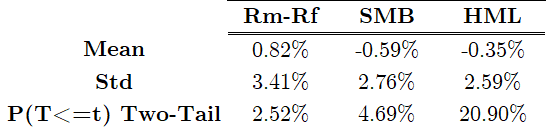
\includegraphics[width=0.45\linewidth]{A1.png}
	\label{fig:label}
\end{figure}

\noindent Also, it was observed that the signs of our observed mean SMB and HML values are in contrast with what Fama and French (1993) observed, a phenomenon which is further investigated in Section 7. The negative mean SMB reading was found to be statistically significant at the 5\% level, albeit mildly so, while the negative  mean HML reading was found to be statistically indifferent from 0 at the 5\% level. 


\noindent \textbf{The Dependent Variables}   

\noindent The table below (Table 2) lists the average annual number of firms in each portfolio over our sample period. Based on these averages, 61.7\% of firms lie in the union of smallest cap quintile and lowest BE/ME quintiles (as underlined).

\begin{figure}[h]
	\centering
	\caption*{Table 2: Average Number of Firms in Quintile-Based Portfolios}
	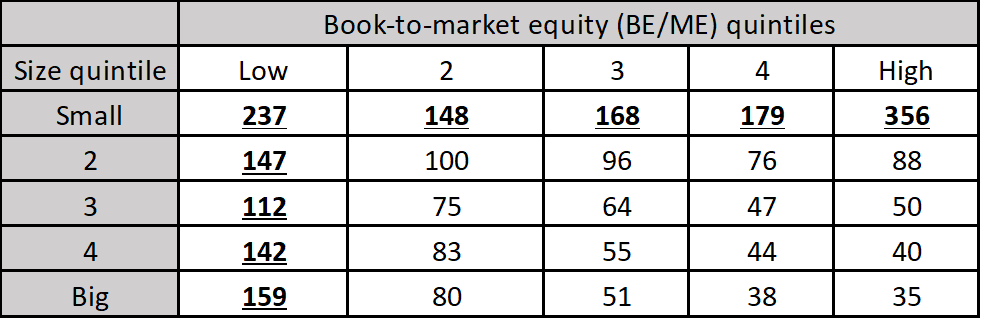
\includegraphics[width=0.5\linewidth]{A3.png}
	\label{fig:label}
\end{figure}

\noindent The table below (Table 3) denotes the average monthly excess return for the 25 quintile-based portfolios over our sample period. We observed a moderate (but in some cases inconsistent) trend of excess portfolio returns increasing with size quintiles. There was also an observed moderate trend of excess portfolio returns decreasing with BE/ME quintiles for Size quintiles 2 through 5.

\begin{figure}[h]
	\centering
	\caption*{Table 3: Mean of Monthly Eccess Return}
	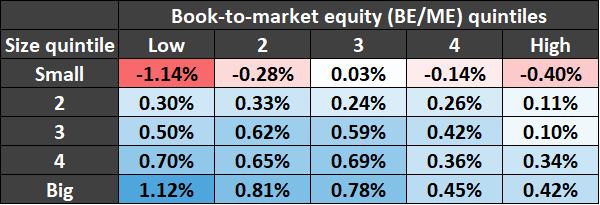
\includegraphics[width=0.48\linewidth]{A4.png}
	\label{fig:label}
\end{figure}

\section{Time-Series Regression Results}

\noindent An outline of the results of our linear regression study is summarised in Table 4. We were unable to reject our null hypothesis of $a=0$ for all but one of our 25 quintile-based portfolios (S1B1, as highlighted). This result was encouraging as a starting point as it implies a near-absence of abnormal returns in Fama and French's (1993) three-factor model over the sample period, lending some credence to our case supporting the model's ability to explain stock return variations. 

\begin{figure}[h]
	\centering
	\caption*{Table 4: Regression Summary for FF3 Model 2011-2018}
	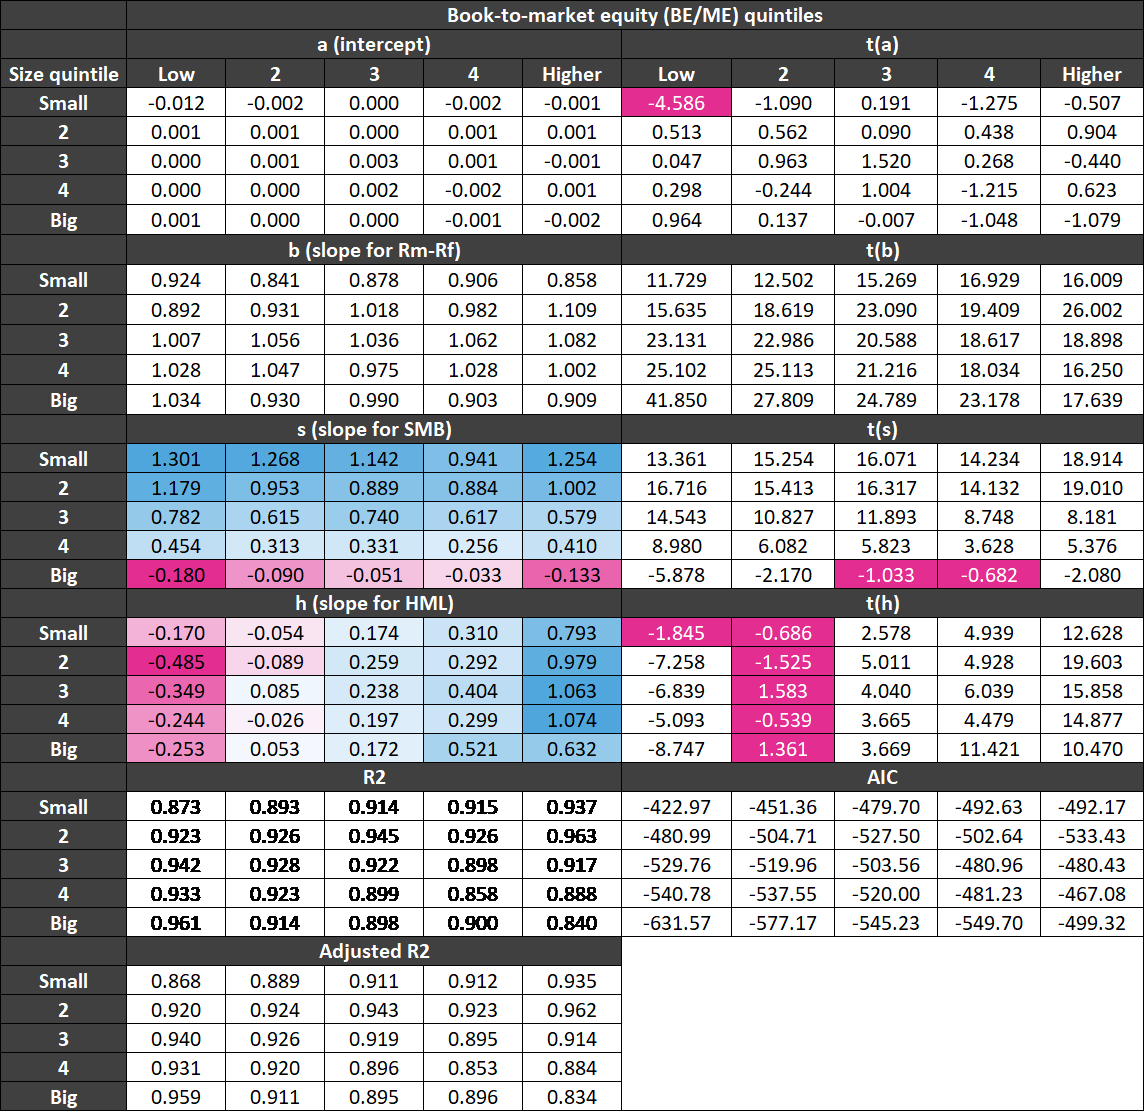
\includegraphics[width=0.9\linewidth]{A5.png}
	\label{fig:label}
\end{figure}

\noindent Devling deeper into the individual slope coefficients of the explanatory variables, we found that the t-test results for slope coefficients $b$ allowed for the rejection of null hypothesis $b=0$. As anticipated, the values of the slope coefficients $b$ were all observed to be close to 1, suggesting little variations in the sensitivities to the market portfolio (if any) between the 25 quintile-based portfolios. Further, the computed t-statistics for slope coefficients $s$ were mostly large enough for the rejection of the null hypothesis $s=0$, with said coefficients seen to be monotonically decreasing with increasing Size. That said, some relative weak t-values for $s$ were seen for portfolios in the Big quintile (S5). As with the case of $s$, the t-statistics for slope coefficients $h$ were mostly large enough for the rejection of the null hypothesis $h=0$, though relatively weak t-statistics were observed for the second BE/ME quintile (B2). $h$ was seen to be increasingly monotonically with increasing BE/ME. Also, the R-squared and adjusted R-squared values for all the regressions run were observed to be extremely significant too.\\

\noindent We also ran a regression study using the standard CAPM in order to highlight the superiority of Fama and French's (1993) three-factor model over the standard one-factor CAPM in terms of explanatory power over U.S. stock returns. Results are tabulated below (Table 5). Generally, the magnitudes of the t-statistics for the intercept term $a$ are much greater than they what we observed from regressions run using the three-factor model, implying that the CAPM alone may not well explain most of variations in U.S. stock returns. Further, the intercept terms $a$ were seen to be increasing with Size, in line with our observed negative mean SMB reading and suggesting that a Size effect may well be in play over our sample period (Banz also noted a size effect in his 1981 study, though his results were in favour of Small firms). The lower R-squared and adjusted R-squared readings computed for regressions run using the CAPM compared to the ones run using the three-factor model also point to the superiority of the latter. Further, regressions run using the three-factor model resulted in lower AIC values compared to those run using the CAPM, suggesting that the three-factor model's incremental explanatory power comes without offsetting overfitting.

\begin{figure}[h]
	\centering
	\caption*{Table 5: Regression Summary for CAPM 2011-2018}
	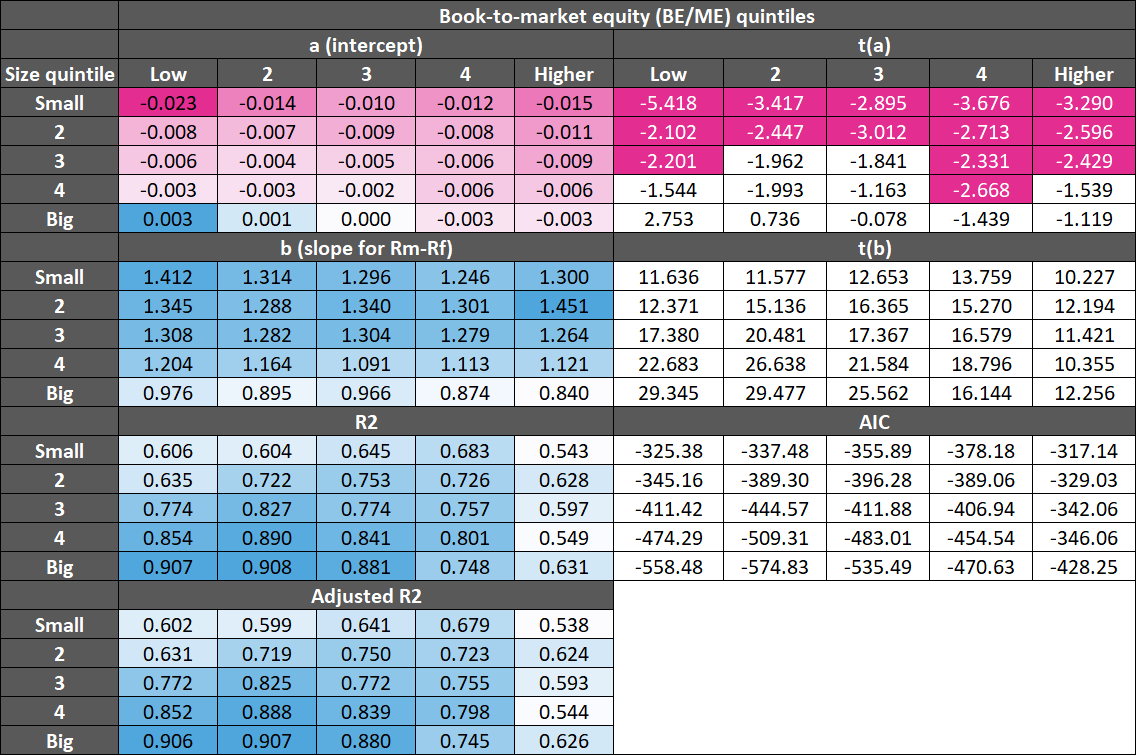
\includegraphics[width=0.9\linewidth]{A6.png}
	\label{fig:label}
\end{figure}

\newpage

\section{SMB, HML and UMD: A Deeper Dive}


\noindent While our findings are generally in line with and supportive of the three-factor model first introduced by Fama and French (1993), a point of divergence arises from our observed mean values of SMB and HML over our sample period. We observed mean values of -0.59\% (statistically significant at the 5\% level) and -0.35\% (statistically insignificant at the 5\% level) for our SMB and HML values respectively, which comes in contrast to Fama and French's (1993) observed mean values of 0.27\% and 0.40\%, especially with regards to the signs of the means. The sign of our observed mean $R_m - R_f$ factor is in line with the one observed in original Fama and French (1993) study. We also look into an additional factor, Up Minus Down (UMD), a proxy for stock return momentum, in this section.\\

\noindent To further examine the behaviour of the SMB, HML and UMD factors over time and how the mean factor realisations can possibly diverge, we treated the factor realisations as actual portfolio returns and tracked the cumulative returns of the constructed portfolios over time. \\

\noindent For this purpose, we utilised monthly Fama-French Factors data between January 1929 to December 2018 provided by WRDS and plotted the cumulative returns of the respective portfolio over this extended sample period. Also, given how monthly SMB, HML and UMD factor realisations tend to have a high level of noise from month to month, we used 7-year rolling averages of the SMB, HML and UMD readings as a gauge of the changes in the broader trends of the respective time series.\\

\noindent \textbf{The SMB Factor}

\noindent For the SMB factor, we found that the factor realisations do not exhibit consistently positive readings over our sample period, though said SMB readings are, on average, mildly positive (at 0.21\%). When using the SMB factor as a proxy, we also observed that the small-firm effect highlighted by Banz (1981) quickly dissipated and even reversed in the years following the publication of his findings, though these two events may have had happened by mere coincidence.

\begin{figure}[h]
	\centering
	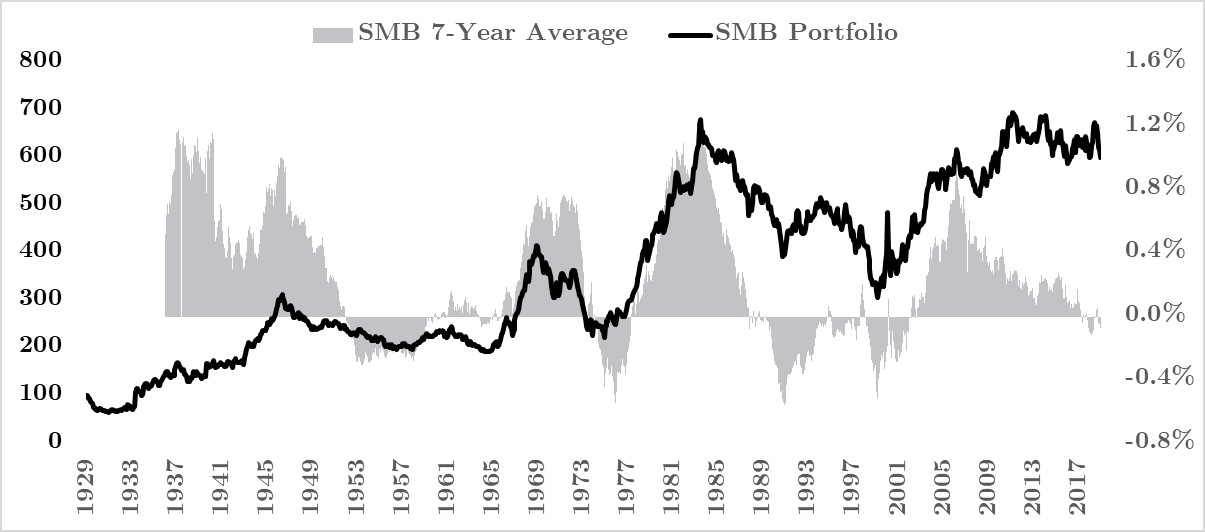
\includegraphics[width=0.9\linewidth]{SMB01}
	\caption*{Fig 01: SMB Portfolio \& Rolling 7-Year Average SMB Returns}
	\label{fig:label}
\end{figure}

\noindent The rolling 7-year SMB average plotted in Fig 01 (grey column chart) shows how the SMB factor realisations have trended in and out of positive territories over our extended sample period. The fluctuations in the level of our constructed SMB Portfolio (blue line chart in Fig 01, starting portfolio size = 100) also highlight the earlier-mentioned point, though the net gain the portfolio has clocked over the extended sample period suggests that SMB factor realisations are still on average, positive. The sample period used in our main study (July 2011 - December 2018) happens to denote a time period when rolling 7-year average SMB factor realisations have once again flipped over to the negative regions, thus explaining the divergence between our observed mean SMB and that of Fama and French (1993).

\begin{figure}[h]
	\centering
	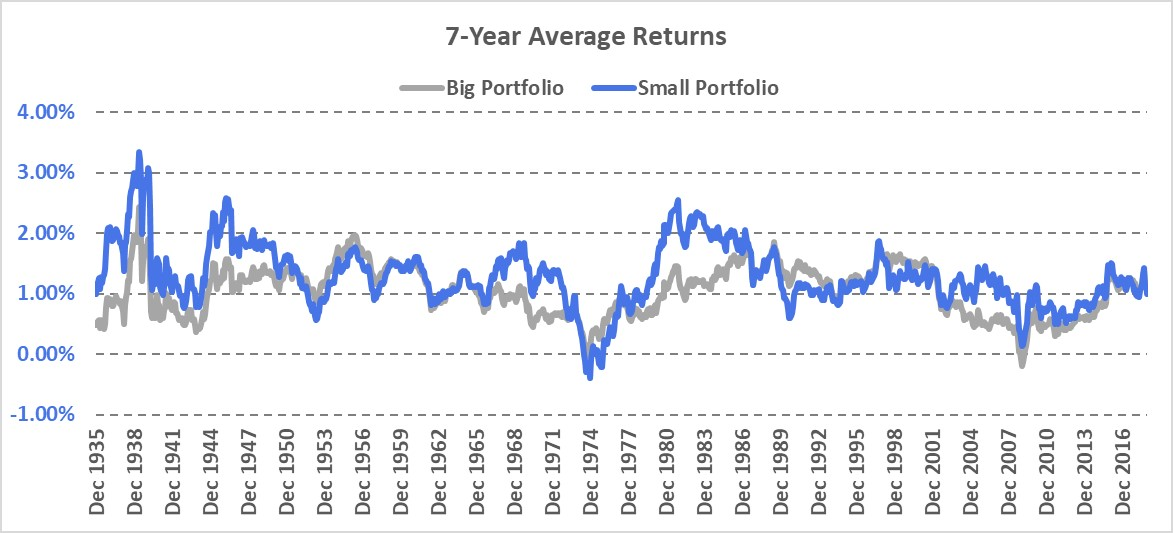
\includegraphics[width=0.9\linewidth]{SMB02}
	\caption*{Fig 02: Small Portfolio vs. Big Portfolio}
	\label{fig:label}
\end{figure}

\noindent Delving deeper, we found that the main driver behind the recent downtrend in rolling 7-year average SMB factor realisations stem mainly from rolling 7-year Big portfolio returns (grey line chart in Fig 02) seeing higher returns growth than rolling 7-year Small portfolio returns (blue line chart in Fig 01), thus gradually closing and even reversing the Small Minus Big (SMB) gap.  It remains to be seen when the long SMB play will be back in vogue, if ever. A summary of descriptive statistics of the SMB factor and our constructed SMB portfolio can be found below (see Table 07).

\newpage

\begin{figure}[h]
	\centering
	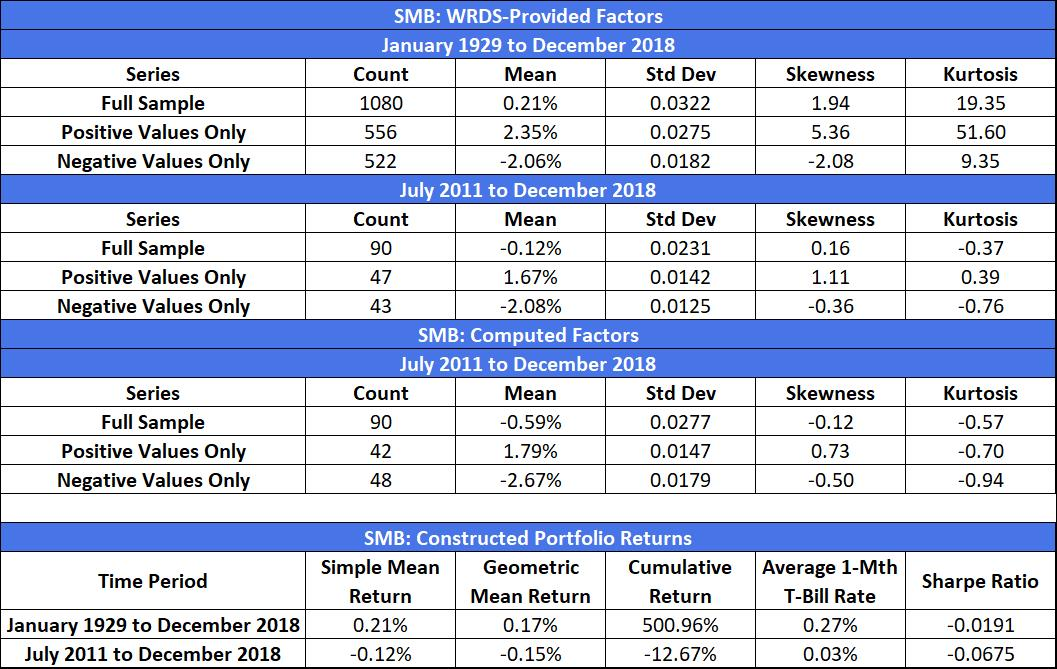
\includegraphics[width=0.8\linewidth]{SMB03}
	\caption*{Table 07: SMB Factor Summary Statistics}
	\label{fig:label}
\end{figure}

\noindent \textbf{The HML Factor}

\noindent Like the SMB factor, the HML factor was observed to exhibit mildly negative mean readings for the period between July 2011 and December 2018, though the HML factor's mean reading of -0.10\% is deemed to be statistically indifferent from 0 at the 5\% significance level. Further, the HML factor was seen to have displayed more consistently and persistently positive readings over the extended sample period of between January 1929 and December 2018 compared to the SMB factor.

\begin{figure}[h]
	\centering
	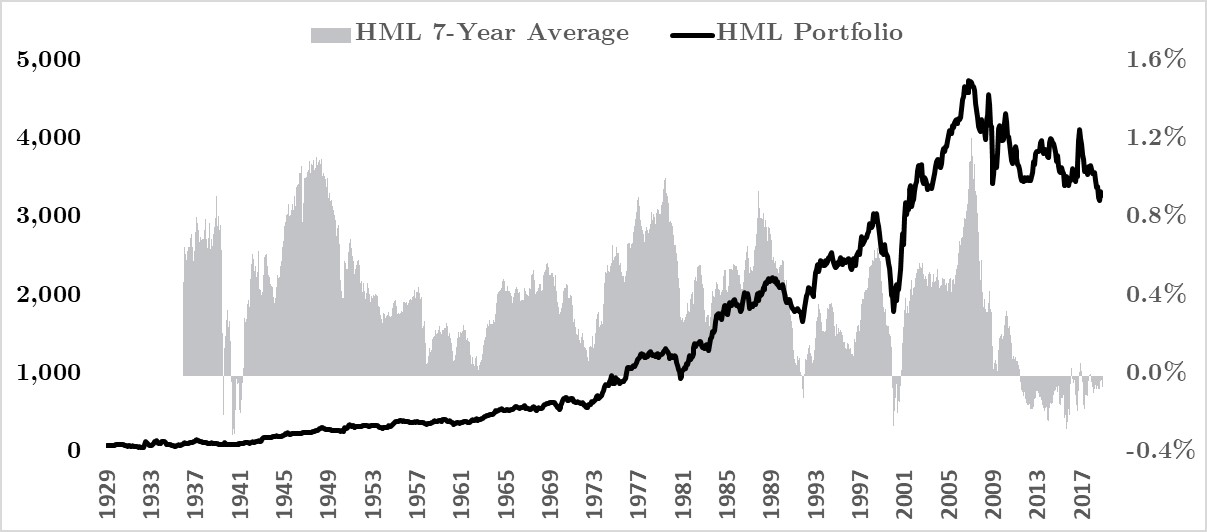
\includegraphics[width=0.9\linewidth]{HML01}
	\caption*{Fig 03: HML Portfolio \& Rolling 7-Year Average HML Returns}
	\label{fig:label}
\end{figure}

\noindent This inference can be drawn from lesser observed instances of negative rolling 7-year average HML factor readings (consistency) and longer streaks of positive rolling 7-year average HML factor readings (persistence) when compared to those of the SMB factor. This makes the unravelling of the HML factor's positive readings over the recent decade all the more an unprecedented one, which also explains the divergence between our observed mean HML and that of Fama and French (1993). 

\begin{figure}[h]
	\centering
	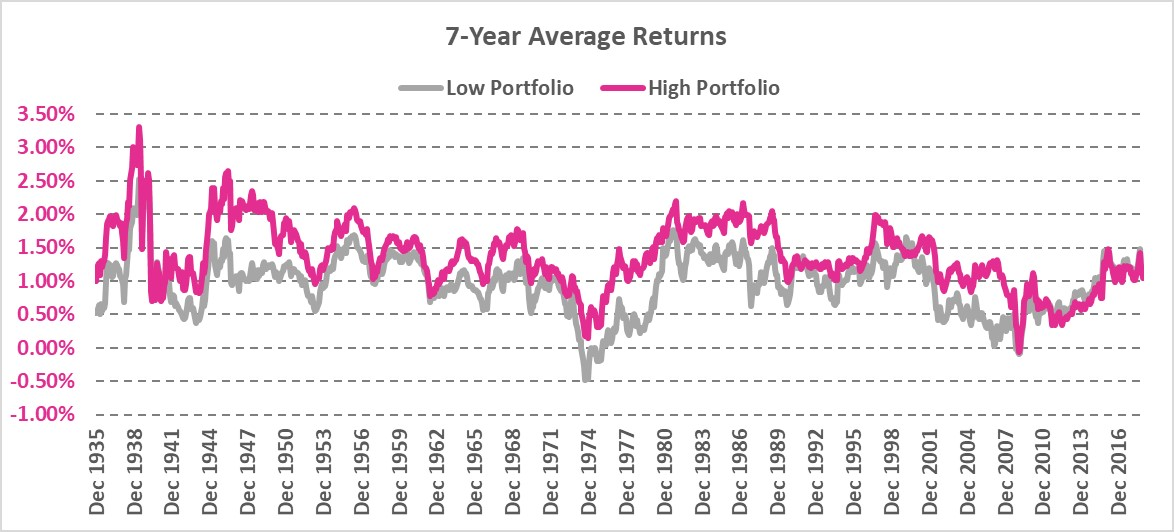
\includegraphics[width=0.9\linewidth]{HML02}
	\caption*{Fig 04: High Portfolio vs. Low Portfolio}
	\label{fig:label}
\end{figure}

\noindent It was also observed that our constructed HML portfolio has grossly outperformed our constructed SMB portfolio over the extended sample period in terms of nominal returns. The HML portfolio clocked 3,200.59\% returns while the SMB portfolio only clocked 500.96\%, with the latter's Sharpe ratio coming up as negative for returns over the extended sample period. With that said, both long SMB and long HML strategies have fallen short during our original sample period of between July 2011 to December 2018. A summary of descriptive statistics of the HML factor and our constructed HML portfolio can be found below (see Table 08).

\begin{figure}[h]
	\centering
	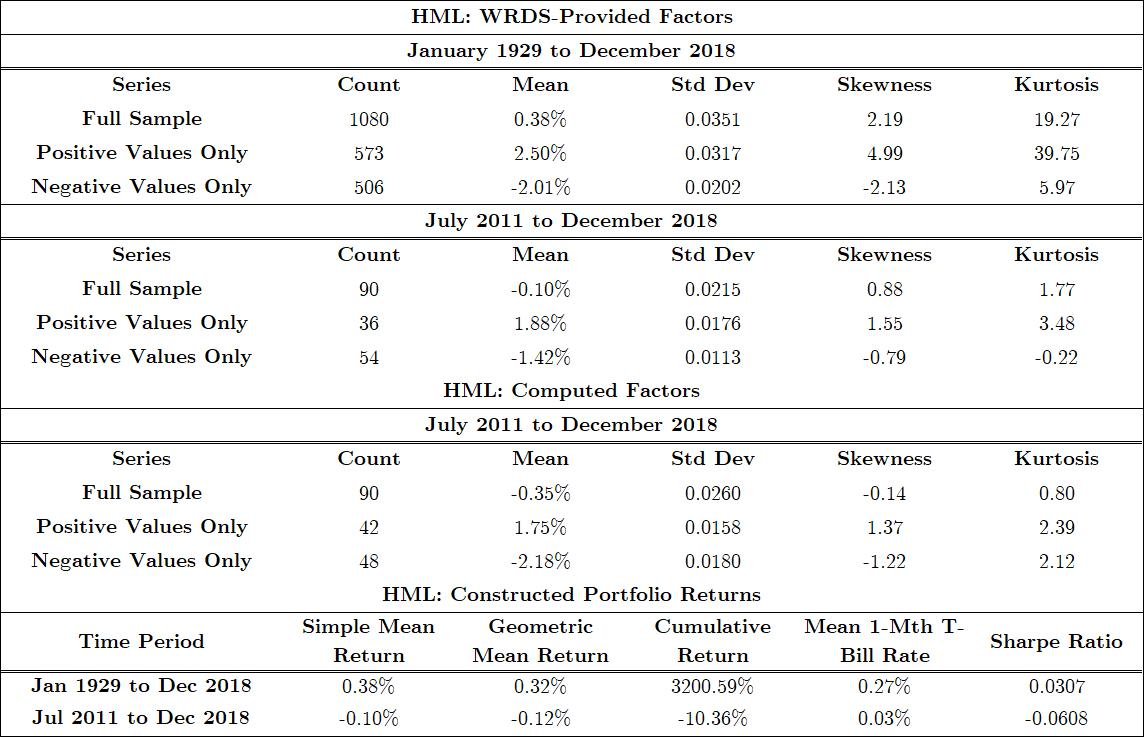
\includegraphics[width=0.8\linewidth]{HML03}
	\caption*{Table 08: HML Factor Summary Statistics}
	\label{fig:label}
\end{figure}

\newpage

\noindent \textbf{The UMD Factor}

\noindent We also looked at one of the additional stock market factors introduced and popularised by Carhart (1997): the momentum factor (UMD). As with the case of the SMB and HML factors, we constructed a UMD portfolio and the rolling 7-year average of UMD readings using data supplied by the WRDS and tracked their fluctuations over the extended sample period.

\begin{figure}[h]
	\centering
	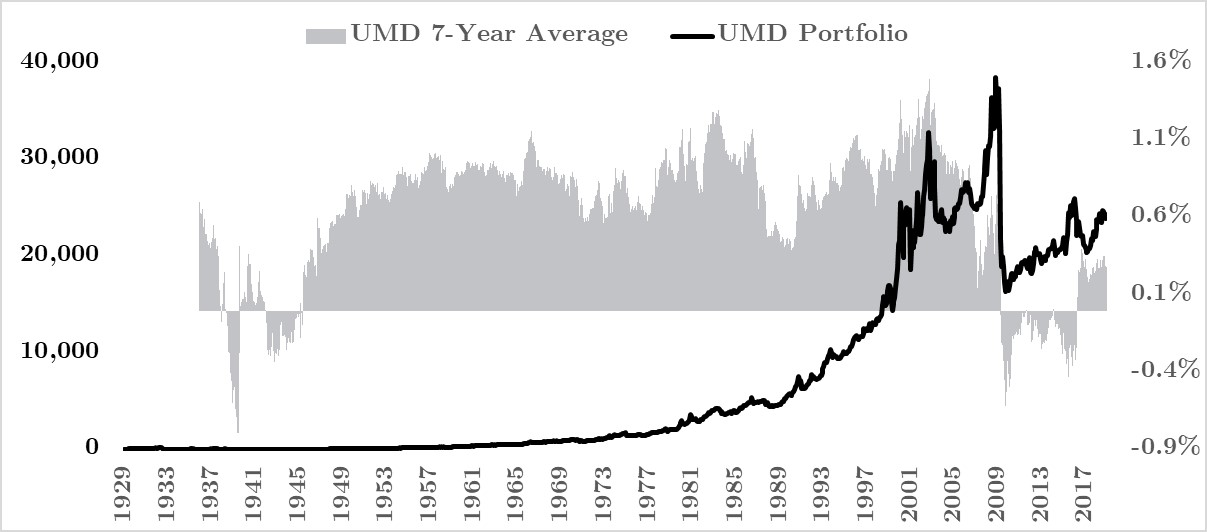
\includegraphics[width=0.9\linewidth]{UMD01}
	\caption*{Fig 05: UMD Portfolio \& Rolling 7-Year Average UMD Returns}
	\label{fig:label}
\end{figure}

\noindent Like the HML factor, it was observed that the UMD factor is consistently and persistently positive given the relatively high frequency of observed instances of positive rolling 7-year average UMD factor readings (consistency) and the long streaks of positive rolling 7-year average UMD factor readings (persistence). Also, like the SMB and HML factors, we observed an unravelling of the long UMD play in the recent decade, though said unravelling took place relatively earlier from April 2009 and has already recovered since April 2016. 

\begin{figure}[h]
	\centering
	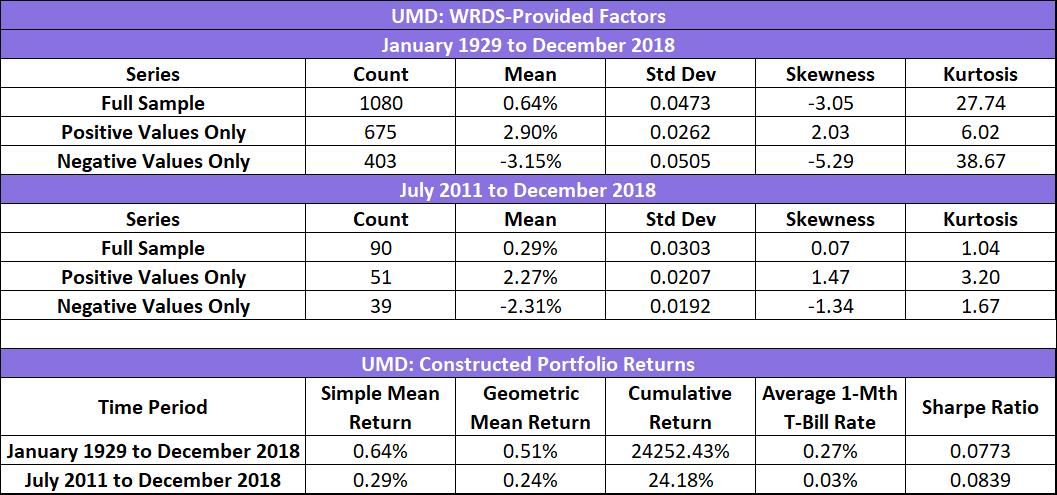
\includegraphics[width=0.8\linewidth]{UMD02}
	\caption*{Table 09: UMD Factor Summary Statistics}
	\label{fig:label}
\end{figure}

\noindent In terms of cumulative returns, the long UMD play has grossly outperformed both the long SMB play and the long HML play, with cumulative nominal returns of 24,252.43\% observed over the extended sample period and 24.18\% over the original sample period. On a risk-adjusted basis and in terms of Sharpe ratios, the long UMD outperforms the long SMB play and the long HML play too. A summary of descriptive statistics of the UMD factor and our constructed UMD portfolio can be found above (see Table 09).


	\section{Conclusion} % Numbered section
	\noindent In our view, we have accomplished our research objective to disprove our null hypothesis and support the case that the Fama and French (1993) three-factor model does significantly explain the returns of stocks listed on the NYSE, NASDAQ and AMEX for the period between July 2011 and December 2018. This view is well-supported by the extremely high and significant adjusted R-squared values obtained as a result of our regression study on the constructed quintile-based portfolios.\\
	
	\noindent We were also able to highlight the three-factor model's superiority over the one-factor CAPM by way of the former's superior adjusted R-squared and AIC results over the latter's. The numerous statistically significantly negative intercept $a$ terms found in our CAPM regression study, a phenomenon not seen in our three-factor model regression study, also suggests that excess market returns alone are not sufficient to explain variations in stock returns, and that the three-factor model may have done the job of better explaining them. Further, we managed to obtain a few possible explanations for our divergent mean SMB and HML readings from Fama and French's (1993) original study, which in no way weakens our case supporting the three-factor model but rather highlights a shift in the profitability of certain thematic plays in recent times.\\
	
	\noindent Overall, it was interesting to note that Fama and French's (1993) three-factor model continues to be relevant, even in more modern times and despite the rise of other viable stock return factors to prominence. The study of factor-based modelling of stock returns continues to evolve, and we will continue to keep our eyes peeled for fresh developments in this space.

	\section{References} % Numbered section
	\begin{itemize}
		\item Markowitz, H. (1952). Portfolio selection. The Journal of Finance, 7(1), 77-91.
		\item Sharpe, W. (1964). Capital asset prices: A theory of market equilibrium under conditions of risk. Journal of Finance, 19(3), 425-442.
		\item Lintner, J. (1965). The valuation of risk assets and the selection of risky investments in stock portfolios and capital budgets. Review of Economics and Statistics, 47(1), 12-37.
		\item Fama, E., \& French, K. (1993). Common risk factors in the returns on stocks and bonds.Journal of Financial Economics, 33(1), 3-56..
		\item Black, Fischer. Michael C. Jensen. and Myron Scholes. 1971. The capital asset pricing model: Some empirical tests. in: M. Jensen. ed.. Studies In the theory of capital markets (Praeger, New York, NY).
		\item Fama. Eugene F. and Kenneth R. French. 1992a. The cross-section of expected stock returns.Journal of Finance 47, 427 - 465.
		\item Fama. Eugene F. and Kenneth R. French. 1992b. The economic fundamentals of size and book-to-market equity. Working paper (Graduate School of Business. Cniversity of Chicago. Chicago. IL).
		\item Elton; Gruber; Blake (1996). "Survivorship Bias and Mutual Fund Performance"
		\item Banz. Rolf W.. 1981. The relationship between return and market value of common stocks, Journal	of Financial Economics 9. 3-15.
		\item Bhandari. Laxmi Chand. 1983. Debt,equity ratto and e.xpected common stock returns: Empirical evidence, Journal of Finance 43. 507-528.
		\item Rosenberg. Barr, Kenneth Reid. and Ronald Lanstein. 1985. Persuasive evidence of market inefficiency.Journal of Portfolio Management Il. 9-17.
		\item Stattman D (1980): Book values and stock returns. The Chicago MBA: A Journal of Selected Papers,4,25–45. 
		\item Basu. Sanjoy. 1983. The relationship between earnings yield. market value. and return for NYSE common stocks: Further evidence. Journal of Financial Economics 12, 129-156.
		\item Daniel, K., \& Titman, S. (1997). Evidence on the characteristics of cross sectional variation in stock returns
		\item Davis, J., Fama, E.,\& French, K. (2000). Characteristics, covariances and average returns: 1927-97. Journal of Finance, 55(1), 389-406
		\item Fama. Eugene F. and Kenneth R. French. 1996. Multifactor Explanations of Asset Pricing Anomalies. Journal of Finance, 51(1), 55--84
		\item Pastor, L., Stambaugh, R.F., 2003. Liquidity risk and expected stock returns. Journal of Political Economy 111, 642–685.
		\item A five-factor asset pricing model. Journal of Financial Economics 116, 1–22.
		\item Hou, K., Xue, C., Zhang, L., 2015. Digesting anomalies: An investment approach. Review of Financial Studies 28, 650–705.
	\end{itemize}


\end{document}
© 2019 GitHub, Inc.
Terms
Privacy
Security
Status
Help
Contact GitHub
Pricing
API
Training
Blog
About
